\chapter{Model Development}\label{ch:model_development}
In this chapter two models are developed based on the simple LSTM model from the silicon-valley-data-science RNN tutorial \cite{rubashkin2017}. Firstly these models (including their simple LSTM model) will be trained and tested on a small data set with the numbers:\\\\
$\left\{zero, one, two, three, four, five, six, seven, eight, nine \right\}$,\\\\
the same data used in Chapter \ref{ch:machine_learning} for the parameter comparison. After that, the best performing model shall be picked for a more detailed discription (with code) and futher trainig with a bigger data set of the english language. 

\section{Neural Network Comparison}

\begin{table}[H]
\centering
	\caption{Models.}
	\begin{tabular}{ l  c }
	Model1 -\tikzcircle[pink, fill=pink]{3pt}- &
	(Their simpleLSTM Model)\\
	Model2 -\tikzcircle[red, fill=red]{3pt}- &
	(Our simpleLSTM Model)\\
	Model3 -\tikzcircle[turquoise, fill=turquoise]{3pt}- &
	(Our BiRNN Model)\\
	\end{tabular}
	\label{tab:3_models}
\end{table}


\begin{table}[H]
\centering
    \caption{Parameter values of the three model.}
    \begin{tabular}{| l | c | c | c | c |} 
    \hline
        Parameters & 
        Model1 -\tikzcircle[pink, fill=pink]{3pt}- &
        Model2 -\tikzcircle[red, fill=red]{3pt}- &
        Model3 -\tikzcircle[turquoise, fill=turquoise]{3pt}-\\
    \hline
        Batch Size & 
        50 \hfill 20 \hfill 20 & 
        50 \hfill 20 \hfill 20 & 
        50 \hfill 20 \hfill 20 \\
    \hline
        Dropout & 
        0.05 & 0.05 & 0.05 \\
    \hline
        Learning Rate & 
        0.001 & 0.001 & 0.001 \\ 
    \hline
    \end{tabular}
    \label{tab:3models_tab}
\end{table}

\begin{figure}[H]
	\centering
	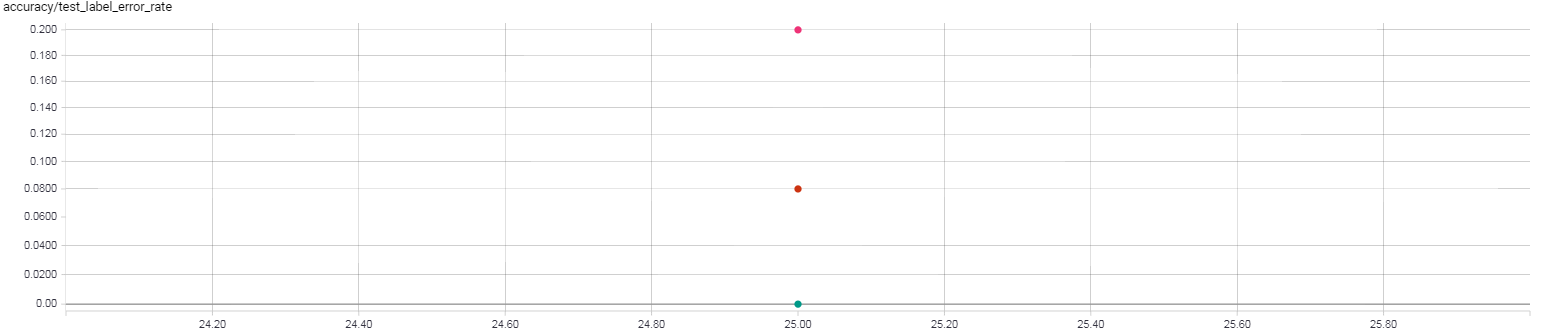
\includegraphics[width=\textwidth]		
	{model_development/3models_comparison/test_error_rate_3models}
	\caption{Test error rate.}
\end{figure}

\begin{figure}[H]
	\centering
	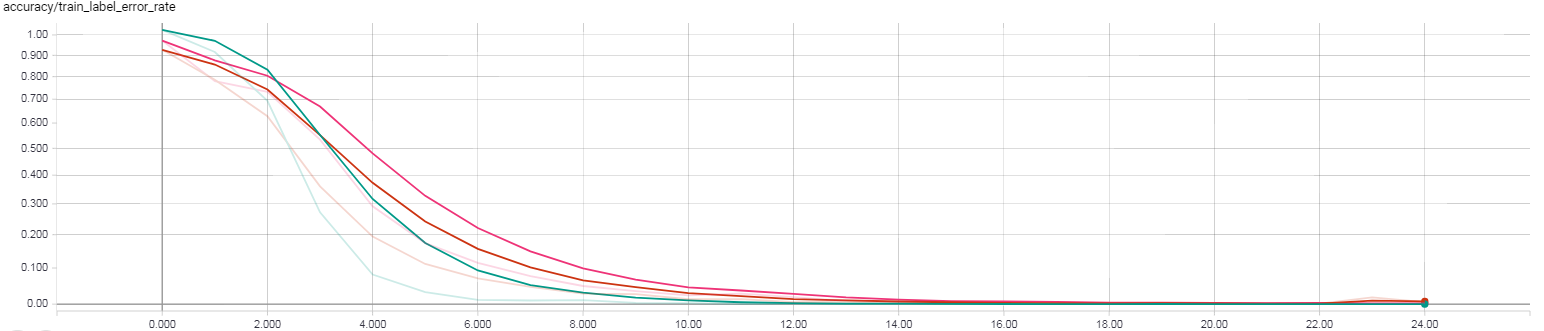
\includegraphics[width=\textwidth]		
	{model_development/3models_comparison/train_error_rate_3models}
	\caption{Training error rate.}
\end{figure}

\begin{figure}[H]
	\centering
	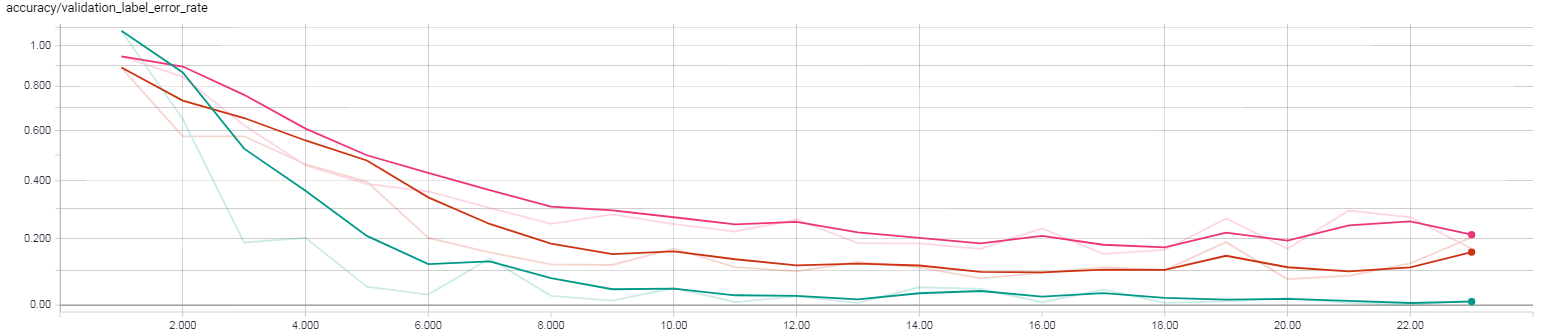
\includegraphics[width=\textwidth]		
	{model_development/3models_comparison/validation_error_rate_3models}
	\caption{Validation error rate.}
\end{figure}

\begin{figure}[H]
	\centering
	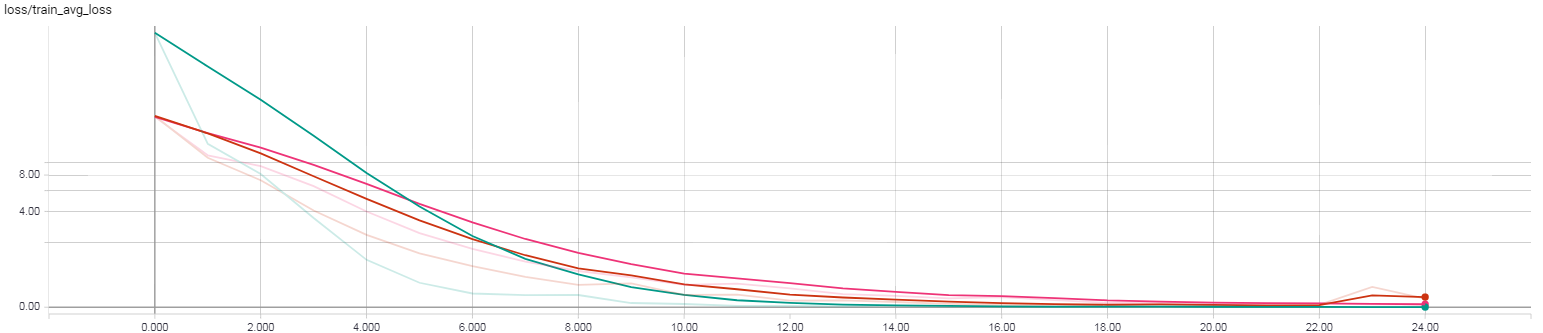
\includegraphics[width=\textwidth]		
	{model_development/3models_comparison/train_avg_loss_3models}
	\caption{Training average loss.}
\end{figure}

\section{Model Description}

Model3 (BiRNN) is better therefore we go into more detail about it...

\begin{figure}[H]
	\centering
	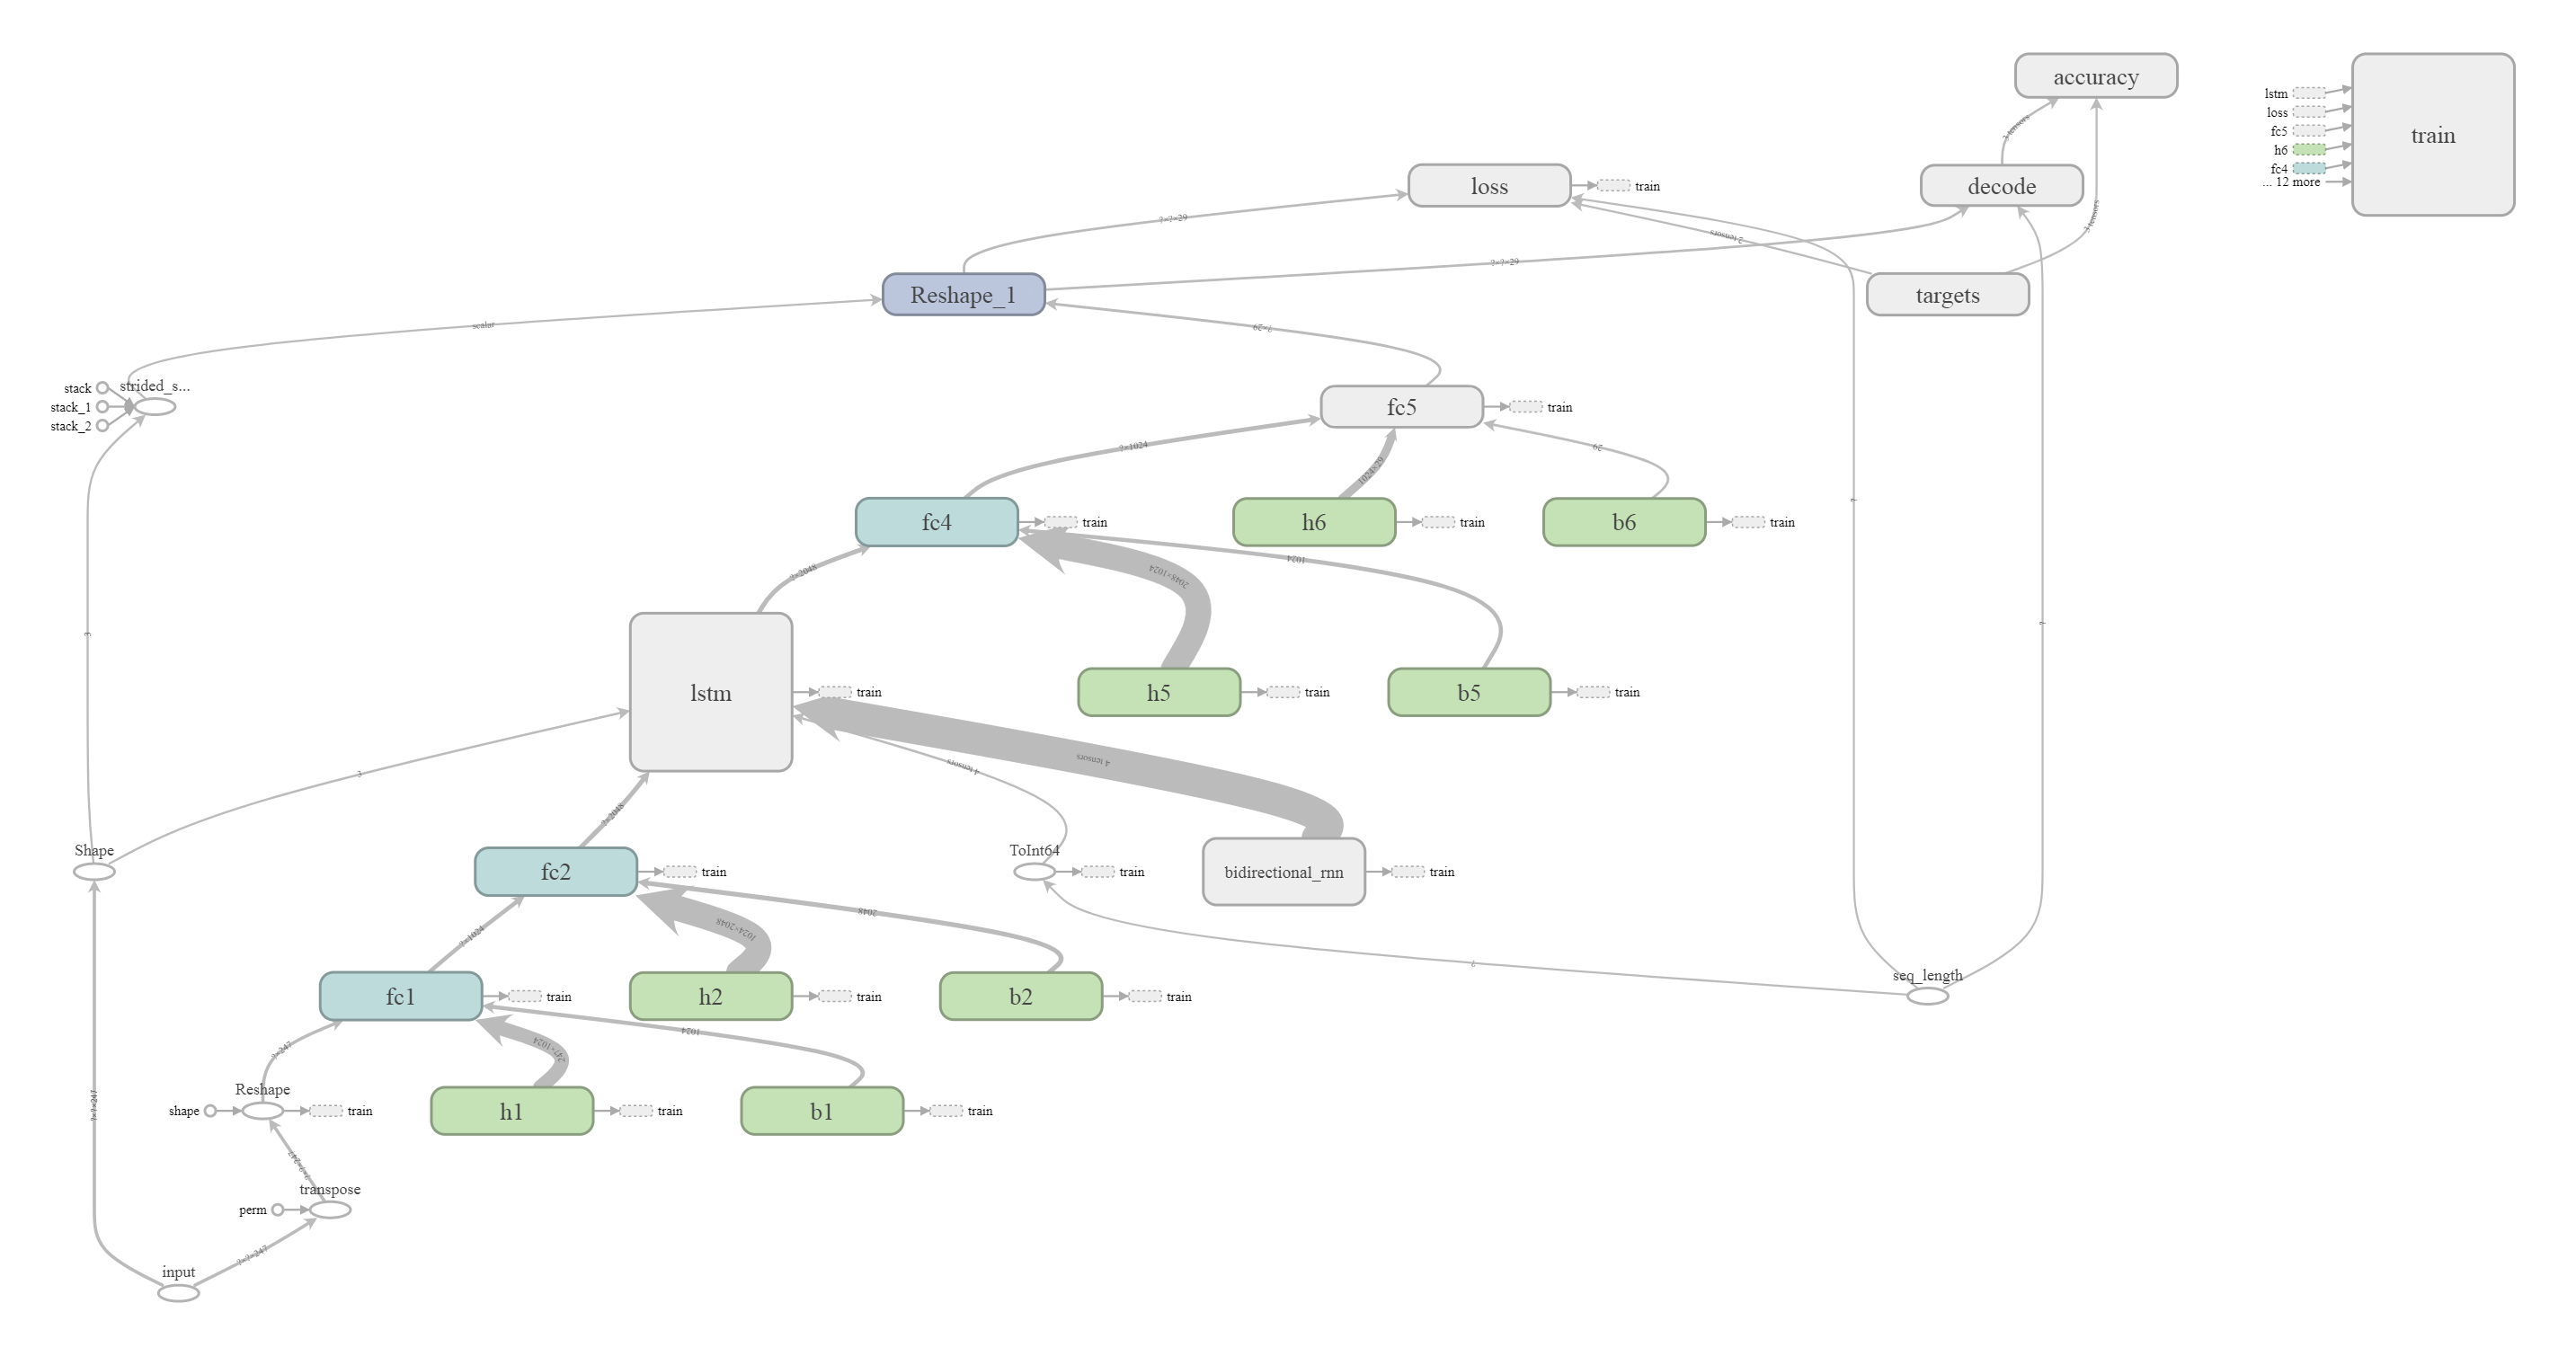
\includegraphics[width=\textwidth]		
	{model_development/birnn_v2_graph}
	\caption{Training average loss.}
\end{figure}